%!TEX root = ../thesis.tex
%*******************************************************************************
%*********************************** First Chapter *****************************
%*******************************************************************************

\chapter{Introduction} \label{Chapter:introduction}  %Title of the First Chapter

\ifpdf
    \graphicspath{{Chapter1/Figs/Raster/}{Chapter1/Figs/PDF/}{Chapter1/Figs/}}
\else
    \graphicspath{{Chapter1/Figs/Vector/}{Chapter1/Figs/}}
\fi


%\section{Background Information}\label{background-information}

As wireless networks evolve through 5G, scaling up spectral density through the use of millimeter-wave frequency bands, Massive MIMO, Non-Orthogonal Multiple Access (NOMA) and dense cells, network designers are looking ahead to the 6G roadmap, anticipating an even more data-driven society where wireless brain-computer interfaces, extended reality, and connected robotics drive 6G networks to handle data rates $10$–$1000\times$ greater than 5G \cite{243}. To scale up spectral efficiency, designers will consider transitioning from traditional orthogonal multiplexing to advanced NOMA schemes, employing innovative air interface multiplexing techniques, more robust forward error correction coding, and even higher-density network deployments in wider bandwidths at higher carrier frequencies. As spectral efficiency is scaled up, 6G system designers will strive to improve \textit{key performance indicators} (KPIs) such as latency, reliability, and energy efficiency of terminals and base-stations while also trying to not compromise one KPI to achieve another. The implementation of algorithms for 6G to optimize data throughput, spectral efficiency, user density, reliability, and latency, operating in wider bandwidths will lead to exponentially more computation than current 5G systems.

In the base station (BS) and cellular infrastructure, 5G RF modem signal processing is based on classical compute concepts which are typically implemented in ASIC, FPGA and GPU/CPU fabrics. However, improvements in classical compute performance are not advancing at an exponential rate as in past years, but are plateauing due to transistors reaching atomic limits \cite{ITRS2015}. Since the design of efficient and fast computational structures is now competing with wireless communication as the most significant challenge for many high-capacity wireless communication systems, it is doubtful that conventional silicon will be able to implement the high spectral performance, low latency, and high-reliability optimization algorithms needed to achieve 6G’s KPIs.

\textit{Quantum computing} is a potentially valuable compute-acceleration tool to address future tradeoffs between performance, latency, and reliability in wireless networks as the 6G roadmap evolves. If quantum computing enables optimal algorithms for computationally heavy optimization problems currently bottleneck achievable network throughput, spectral efficiency could then benefit. The numerous hardware platforms capable of quantum information processing could then combine with other scalable technologies such as millimeter wave and small cells, further increasing spectral efficiency. Due to the linearity of quantum mechanics, quantum computing is fundamentally constrained to rely on reversible operations, which dissipate no heat, except in the initialization and readout phase of the computation. While noisy quantum computation has elements of irreversibility, in the long term quantum computation can in principle reach arbitrarily low power consumption for computations that would be power-hungry if performed classically.
\begin{figure}
    \centering
    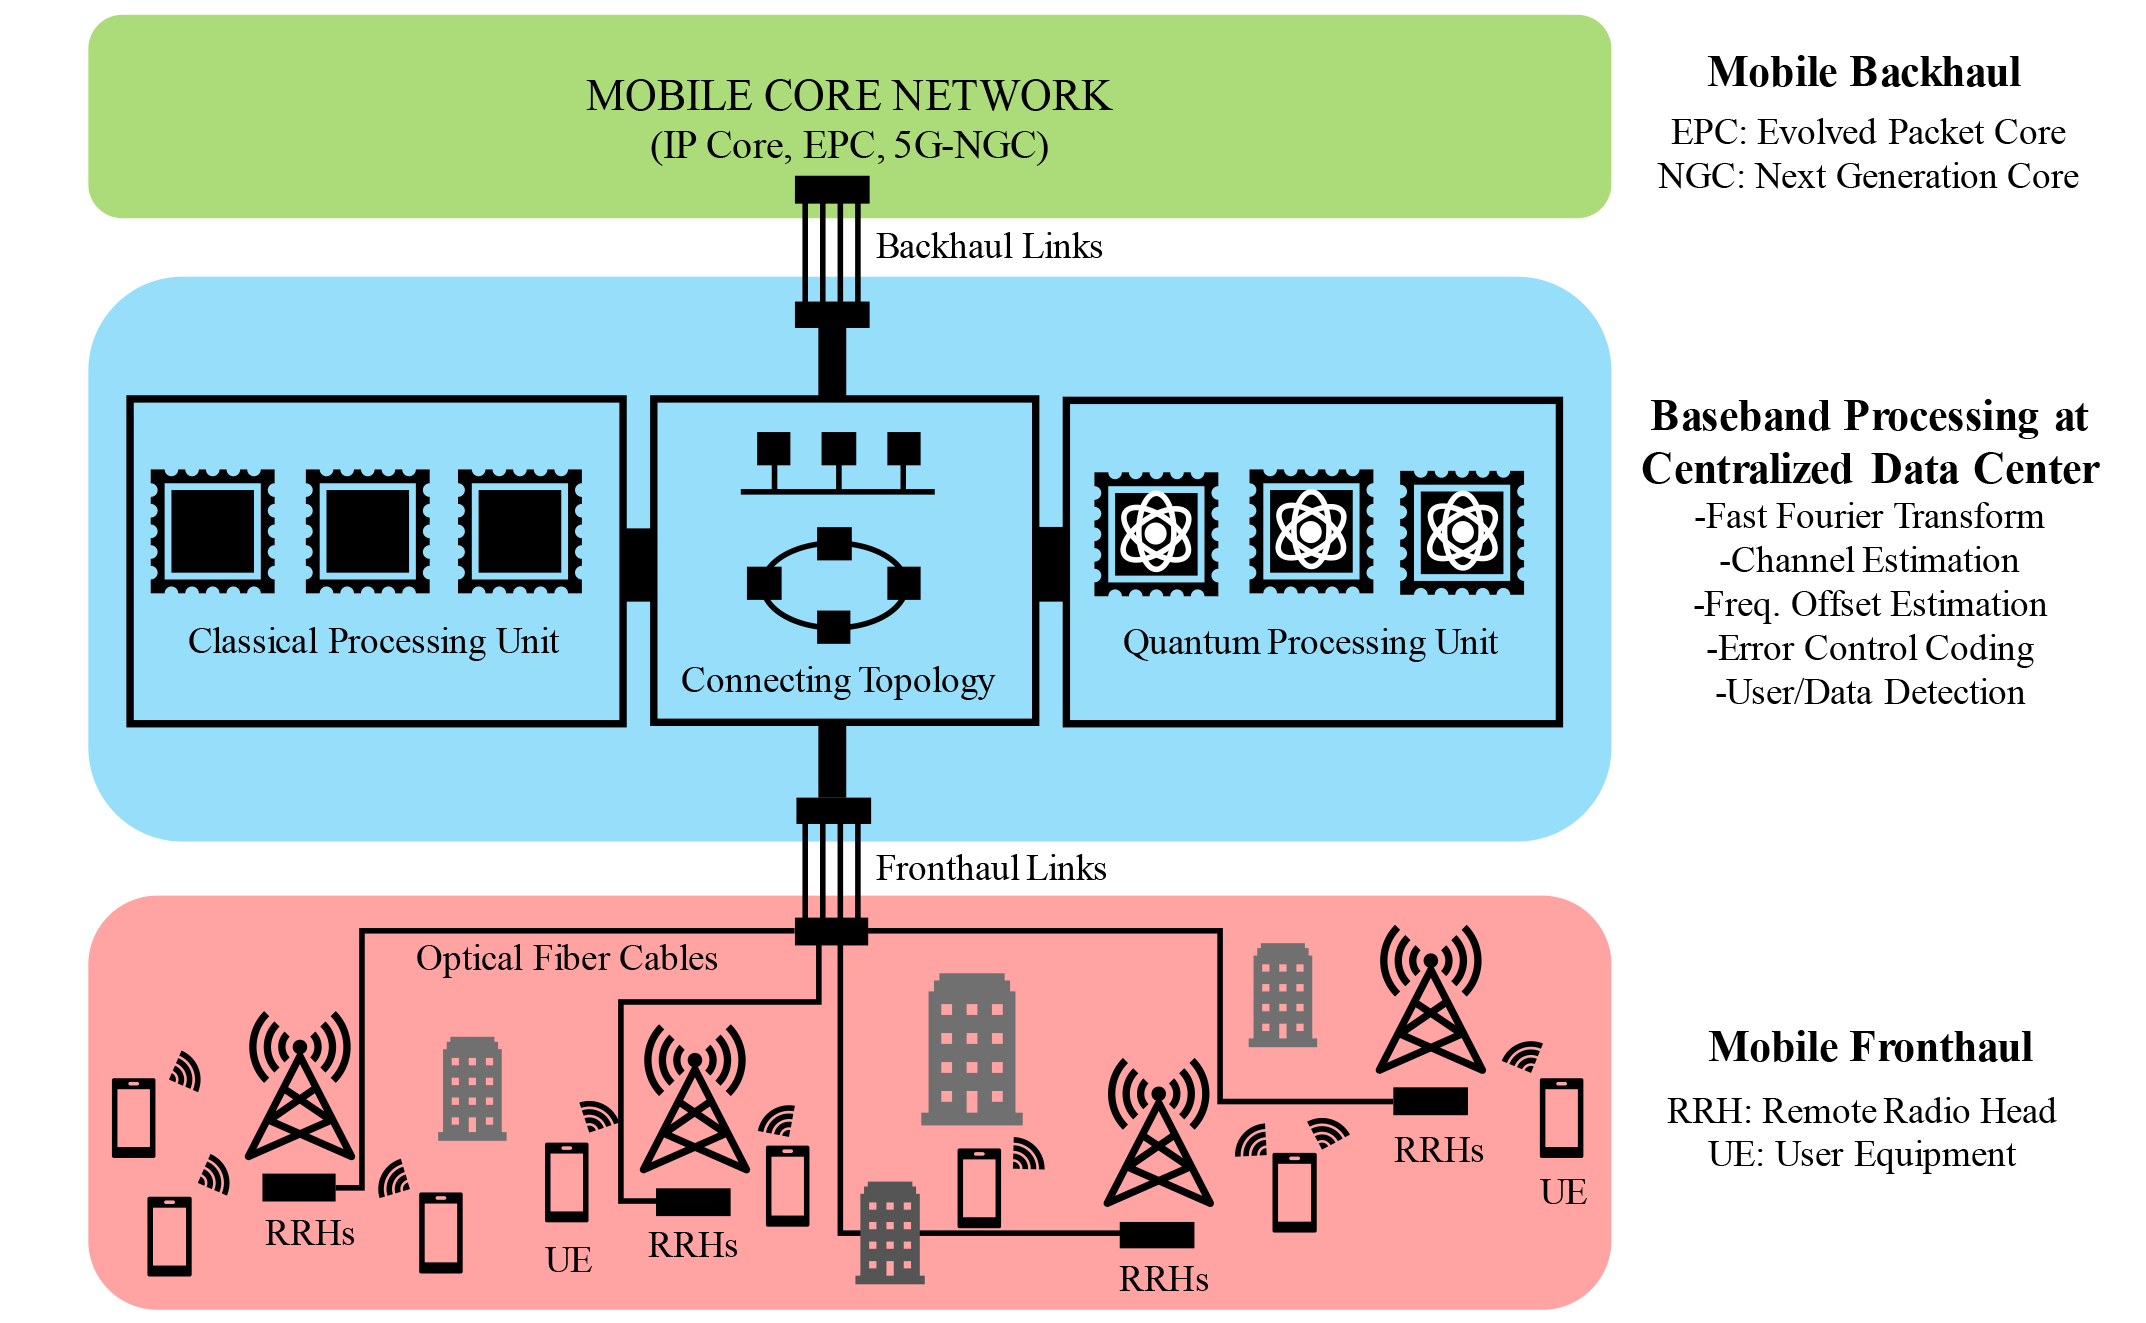
\includegraphics[width=1\linewidth]{Chapter1/qacran.png}
    \caption{A quantum compute-enabled C-RAN system architecture for NextG wireless
networks.}
    \label{fig:qacran}
\end{figure}
Over the last few years, due to advances in nanotechnology and engineering, real-world quantum computers have become commercially available. For wireless networks, recent studies first made use of a quantum annealer, a certain type of analog quantum computing processor, and showed promising results for a quantum-based MIMO detector in centralized radio access networks (C-RAN) \cite{Kim2019} and for a quantum-based Low-Density Parity Check (LDPC) error control decoding \cite{ldpc}, providing guidance of how to make use of the machine and baseline performance metrics. In wireless networks, there are representative optimization problems, including but not limited to the previously studied applications, which suffer from well-known conventional trade-offs between throughput and compute complexity, where optimal solvers are known but very difficult to practically implement considering available hardware and processing time limitations. We expect that overcoming practical issues of these optimization problems existing on current algorithms and/or computer architectures will lead to drastic improvements in wireless communications and networks, achieving optimal performance within a short processing time, making investigation of quantum computing as a potential accelerator a compelling research objective. In our envisioned scenario shown in \autoref{fig:qacran}, quantum processors will be co-located with C-RAN computational resources in a data center, partitioning the compute roles for hundreds of base stations or Remote Radio Heads (RRH) connected via low-latency optical fiber, where quantum computing will take care of computationally-demanding optimization processing that bottlenecks achievable throughput and latency, while classical processors will take care of otherwise tractable processing \cite{kimdwave6g,kimcost}. We believe that the C-RAN embedded quantum processors will have optimized interfaces and information processing architecture to maximize wireless system performance.


\section{Problem Statement}\label{problem-statement}


The demand for faster and more capable video, audio, and teleconferencing applications over the past decade has led to sharp and unprecedented increases in wireless traffic loads at base stations. To address this, \textit{Non-orthogonal multiple access} (NOMA) has emerged as a promising technique to maximize spectral efficiency in modern wireless systems like 5G New Radio cellular networks and beyond. In NOMA, the use of overlapping or the same time and frequency slots for all users has allowed for a significant improvement in the utilization of network resources compared to traditional orthogonal multiple access (OMA) techniques.

From a design standpoint, one of the most efficient architectures to implement advanced 5G technologies is the C-RAN architecture \cite{cran1}. C-RAN offloads most of the physical-layer processing that currently takes place at the BS to a centralized data
center, where it is aggregated with other BSs’ processing on the same hardware, supporting hundreds or thousands of access points. This centralized computation helps in managing the increased complexity and computational load that NOMA introduces, especially in handling multi-user interference, which is crucial for maintaining high data rates and system reliability in NOMA networks.

In practice, however, to fully realize NOMA's potential for throughput and spectral efficiency gains, the system must effectively and efficiently demultiplex mutually-interfering information streams as they arrive. NOMA requires sophisticated signal processing techniques to disentangle these overlapping signals, which often involve the use of successive interference cancellation (SIC) \cite{liu2020noma}. the practical implementation of NOMA, especially in uplink scenarios, faces significant challenges. SIC suffer from high implementation complexity, error propagation in iterative decoding, while the optimal maximum likelihood (ML) suffer from stringent latency requirements that can hinder the performance of NOMA systems.

%Moreover, recent advancements have sought to address these challenges through innovative approaches. Techniques such as deep neural networks for joint channel estimation and signal detection, and alternative interference cancellation strategies like parallel interference cancellation (PIC), have been explored to enhance NOMA's performance. Additionally, the integration of quantum computing, particularly quantum annealing, into NOMA signal detection processes at C-RAN computation centers is being investigated as a potential solution to reduce the computational burden and achieve ultra-low latency in signal processing.

To address these challenges, this project proposes the use of Quantum Annealing (QA) for uplink signal detection in NOMA networks. QA, which runs on specialized quantum computing hardware, offers a novel approach to solving the computationally intensive task of maximum likelihood signal detection, traditionally a bottleneck in high-density NOMA scenarios. By reformulating the signal detection problem as an Ising spin energy minimization problem, QA can be leveraged to perform this task more efficiently and with potentially lower latency than classical algorithms \cite{Gabdulsattarov2023,Kizilirmak2020}.





\section{ Project Objectives}\label{objectives}
The project objectives are summarized as follows:
\begin{itemize}
    \item Study and understand the existing multiplexing schemes, focusing particularly on Non-Orthogonal Multiple Access (NOMA), and compare their efficiencies and applications.
    
    \item Investigate the current techniques proposed for implementing power-domain NOMA (PD-NOMA) and identify their limitations and drawbacks in practical scenarios.
    
    \item Explore the principles of Quantum Annealing (QA) and its applicability in solving complex computational problems, especially those related to signal processing in wireless communications.
    
    \item Apply the Quadratic Unconstrained Binary Optimization (QUBO) transformation to the Maximum Likelihood (ML) detection problem for NOMA systems, as established in prior research, to enable its integration with Quantum Processing Units (QPUs).
    
    \item Study the Bit Error Rate (BER) performance of QA-aided ML Multi-User Detection (MUD) across various modulation schemes and assess how it scales with an increasing number of users.
    
    \item Compare the QA method with other conventional signal detection techniques, including Successive Interference Cancellation (SIC) and brute force solutions for maximum likelihood detection, highlighting the advantages and potential improvements offered by QA.
\end{itemize}


\section{Structure of Report}\label{structure-of-report}

This project is systematically organized into the following chapters to provide a comprehensive exploration of the integration of quantum computing with wireless communications:

\begin{itemize}
    \item \textbf{Chapter 1: Introduction} --- Provides an overview of wireless communications, delineates the problem statement, outlines project objectives, and describes the project's organizational structure.
    \item \textbf{Chapter 2: Towards Non-Orthogonal Multiple Access
for Next-Gen Wireless Networks} --- Discusses the technology, performance, and challenges of Power-Domain NOMA in uplink multi-user detection, critiques the limitations of Successive Interference Cancellation (SIC), and promote for Maximum Likelihood detection as a superior alternative.
    \item \textbf{Chapter 3: Introduction to Quantum Annealing} --- Introduces key concepts of quantum computation, offers a tutorial on using Noisy-Intermediate-Scale Quantum (NISQ) technology, and details quantum annealing (QA), particularly the application of D-Wave systems for practical purposes in wireless communications.
    \item \textbf{Chapter 4: Leveraging Quantum Annealing for
Large NOMA Processing in Centralized
Radio Access Networks} --- Starts with a detailed system model for NOMA, explains the conversion of the NOMA problem into a Quadratic Unconstrained Binary Optimization (QUBO) format, describes its implementation on quantum annealing hardware, and evaluates the system’s performance in optimizing NOMA decoding.
    \item \textbf{Chapter 5: Conclusions and Future Work} --- Summarizes the findings of the project and outlines the potential future directions for extending this research.
\end{itemize}
%********************************** %First Section  **************************************

\nomenclature[z-NOMA]{NOMA}{Non-Orthogonal Multiple Access}
\nomenclature[z-5G]{5G}{Fifth Generation}
\nomenclature[z-6G]{6G}{Sixth Generation}
\nomenclature[z-4G]{4G}{Fourth Generation}
\nomenclature[z-3G]{3G}{Third Generation}
\nomenclature[z-1G]{1G}{First Generation}
\nomenclature[z-2G]{2G}{Second Generation}
\nomenclature[z-RF]{RF}{Radio Frequency}
\nomenclature[z-SINR]{SINR}{Signal-to-Interference-Plus-Noise Ratio}
\nomenclature[z-SNR]{SNR}{Signal-to-Noise Ratio}
\nomenclature[z-UE]{UE}{User Equipment}
\nomenclature[z-KPIs]{KPIs}{Key Performance Indicators}
\nomenclature[z-BS]{BS}{Base Station}
\nomenclature[z-LDPC]{LDPC}{Low-Density Parity Check}
\nomenclature[z-CRAN]{C-RAN}{Centralized Radio Access Networks}
\nomenclature[z-RRH]{RRH}{Remote Radio Heads}
\nomenclature[z-OMA]{OMA}{Orthogonal Multiple Access}
\nomenclature[z-SIC]{SIC}{Successive Interference Cancellation}
\nomenclature[z-QA]{QA}{Quantum Annealing}
\nomenclature[z-PDNOMA]{PD-NOMA}{Power-Domain Non-Orthogonal Multiple Access}
\nomenclature[z-QUBO]{QUBO}{Quadratic Unconstrained Binary Optimization}
\nomenclature[z-QPUs]{QPUs}{Quantum Processing Units}
\nomenclature[z-BER]{BER}{Bit Error Rate}
\nomenclature[z-MUD]{MUD}{Multi-User Detection}
\nomenclature[z-mMTC]{mMTC}{Massive Machine-Type Communications}
\nomenclature[z-URLLC]{URLLC}{Ultra-Reliable Low-Latency Communications}
\nomenclature[z-THz]{THz}{Terahertz}
\nomenclature[z-IoE]{IoE}{Internet of Everything}
\nomenclature[z-SE]{SE}{Spectral Efficiency}
\nomenclature[z-EE]{EE}{Energy Efficiency}
\nomenclature[z-NGMA]{NGMA}{Next Generation Multiple Access}
\nomenclature[z-eMBB]{eMBB}{Enhanced Mobile Broadband}
\nomenclature[z-FDMA]{FDMA}{Frequency Division Multiple Access}
\nomenclature[z-TDMA]{TDMA}{Time Division Multiple Access}
\nomenclature[z-CDMA]{CDMA}{Code Division Multiple Access}
\nomenclature[z-OFDM]{OFDM}{Orthogonal Frequency Division Multiplexing}
\nomenclature[z-VR]{VR}{Virtual Reality}
\nomenclature[z-AR]{AR}{Augmented Reality}
\nomenclature[z-SC]{SC}{Superposition Coding}
\nomenclature[z-IoT]{IoT}{Internet of Things}
\nomenclature[z-MnAC]{MnAC}{Many-Access Channel}
\nomenclature[z-CDNOMA]{CD-NOMA}{Code-Domain Non-Orthogonal Multiple Access}
\nomenclature[z-SCMA]{SCMA}{Sparse Code Multiple Access}
\nomenclature[z-PDMA]{PDMA}{Pattern Division Multiple Access}
\nomenclature[z-RSMA]{RSMA}{Rate Splitting Multiple Access}
\nomenclature[z-SDMA]{SDMA}{Space Division Multiple Access}
\nomenclature[z-DoFs]{DoFs}{Degrees of Freedom}
\nomenclature[z-MUST]{MUST}{Multiuser Superposition Transmission}
\nomenclature[z-CSI]{CSI}{Channel State Information}
\nomenclature[z-MLD]{MLD}{Maximum Likelihood Detection}
\nomenclature[z-QPSK]{QPSK}{Quadrature Phase Shift Keying}
\nomenclature[z-QAM]{QAM}{Quadrature Amplitude Modulation}
\nomenclature[z-MIMO]{MIMO}{Multiple Input Multiple Output}
\nomenclature[z-NISQ]{NISQ}{Noisy-Intermediate-Scale Quantum}
\nomenclature[z-P]{P}{Polynomial}
\nomenclature[z-NP]{NP}{Non-deterministic Polynomial}
\nomenclature[z-AQC]{AQC}{Adiabatic Quantum Computation}
\nomenclature[z-SQUID]{SQUID}{Superconducting Quantum Interference Devices}
\nomenclature[z-QMI]{QMI}{Quantum Machine Instruction}
\nomenclature[z-APs]{APs}{Access Points}
\nomenclature[z-ULNOMA]{UL-NOMA}{Uplink Non-Orthogonal Multiple Access}
\nomenclature[z-BF]{BF}{Brute Force}
\nomenclature[z-QAOA]{QAOA}{Quantum Approximate Optimization Algorithm}
\nomenclature[z-Bbu]{BBU}{Baseband Unit}
\nomenclature[z-sapi]{SAPI}{Solver Application Programming Interface}
\nomenclature[z-RB]{RB}{Resource Block}
\nomenclature[z-PA]{PA}{Power Allocation}